\documentclass[11pt,a4paper]{article}
\usepackage[margin=2.2cm]{geometry}
\usepackage{graphicx,booktabs,amsmath,amssymb,enumitem,array}
\usepackage[hidelinks]{hyperref}
\graphicspath{{../paper/figures/}}
\setlist{itemsep=0pt,topsep=2pt,parsep=0pt}
\setlength{\parskip}{0pt}\setlength{\parindent}{0pt}
\setlength{\textfloatsep}{8pt}\setlength{\intextsep}{6pt}
\newenvironment{experiment}[2]{\subsection{#1}\label{#2}}{}
\newcommand{\Q}{\par\textbf{Question.}\ }
\newcommand{\D}{\par\textbf{What we did.}\ }
\newcommand{\R}{\par\textbf{Result.}\ }
\newcommand{\M}{\par\textbf{What it means.}\ }
\newcommand{\status}[1]{\par\textbf{Status:} #1}
\newenvironment{keybox}[1]{\par\textbf{#1.}\ }{\par}
\newenvironment{warnbox}[1]{\par\textbf{#1.}\ }{\par}
\begin{document}

\begin{center}
{\Large\bfseries PP-HFM: Patient-Private Hierarchical Federated Multimodal Learning}\\[2pt]
Project report: the idea, the system, every experiment and what each one showed\\[2pt]
Samartha H V (Regd.\ No.\ 251580130019) \quad Guide: Dr.\ Shreyas J \quad Industry mentor: Mr.\ Tejas J (Capgemini)\\
MIT Bengaluru (MAHE) \quad Status as of 28 October 2026
\end{center}
This is an internal report, not the paper. Every number is taken from the result files under \texttt{SIMULATORS/results/}; results still being re-run are marked pending.


%======================================================================
\section{The project in one page}

\begin{keybox}{The one-sentence version}
We built a three-tier federated learning system (devices $\rightarrow$ edge servers
$\rightarrow$ cloud) that trains a multimodal clinical model without moving raw
data, and that protects every \emph{patient}, not just every data
\emph{record}, with a mathematically proven differential-privacy guarantee. We
then measured, carefully, what that protection costs.
\end{keybox}

\paragraph{The problem.} Hospitals and IoT devices produce data that cannot leave
the site. Federated learning (FL) solves this: each site trains locally and only
sends model updates. Differential privacy (DP) adds noise so that the updates do
not reveal any individual. But almost every published DP system protects a
\emph{record} (one 10-minute window of sensor data). A patient contributes many
records, around 8 in VitalDB and 28 in eICU. Protecting each record does
\emph{not} protect the patient: if you convert after the fact (``group
privacy''), a guarantee of $\varepsilon \approx 1$ per record becomes
$\varepsilon \approx 8$ per patient, which is almost no protection.

\paragraph{Our answer.} PP-HFM makes the patient the privacy unit from the start.
All of a patient's records are summed into one gradient, that sum is clipped,
and noise is added to it. Each client (hospital) gets its own noise level
calibrated to its own patient count. Every release in the hierarchy (devices,
edges, cloud) is accounted for, and a theorem proves the guarantee.

\paragraph{What we found, in brief.}
\begin{enumerate}
\item \textbf{The system works.} Uplink traffic falls 90.8--96.1\,\%, energy per
round falls 72.3--79.6\,\%, and inference takes at most 2.3\,ms (target was
100\,ms), on all three datasets.
\item \textbf{Patient-level privacy at $\varepsilon = 0.9$ costs no measurable
accuracy on VitalDB} but costs 3.1 AUROC points on eICU, because of the
smallest hospitals.
\item \textbf{The thing that makes strict privacy survivable is pretrained
initialization}, not the trick of privatizing only the model head. A randomly
initialized private model loses 0.19 AUROC; a pretrained one loses 0.004.
\item \textbf{The cost of protecting patients grows with the number of records
per patient, $k$, and then flattens.} This follows the curve $A(1-1/k)$,
and vanishes at $k = 1$, where a patient \emph{is} a record. It was
forecast in advance and tested on a second hospital corpus: the
\emph{shape} transferred, the \emph{size} did not.
\item Several things we expected did \emph{not} hold, and we report them:
the membership-inference attack did not find the big leakage difference we
predicted; private conformal prediction gave useless prediction sets;
fusion did not help on eICU.
\end{enumerate}

%======================================================================
\section{How the project progressed (phases)}

\begin{center}
\small
\begin{tabular}{l p{0.72\textwidth}}
\toprule
Phase & What happened \\
\midrule
1--2 & Literature review and problem definition. Four research gaps identified
(Section~\ref{sec:gaps}); four quantified objectives fixed. \\
3 & Environment: Python stack, NS-3 network simulator (v3.46.1), CloudSim Plus
(v8.5.6) for energy, GPU utilities. \\
4 & Both simulators implemented: network (latency, traffic, reliability) and
edge--cloud resource/energy model. First system-level numbers. \\
5 & The learning system: multimodal model, hierarchical FL, DP, compression,
conformal calibration. All 17 deliverables on VitalDB and WEAR (5 Aug).
Four silent bugs found and fixed. \\
6 & Ablations and baselines: which component does what. Hierarchy
resolved at 6 seeds; pretrained-initialization finding. \\
7 & External validation on eICU (187 hospitals), the $k$-scaling law,
pre-registered tests, paper writing. \\
Fix (22 Oct--) & A flaw in the patient-DP mechanism was found while writing the
proof. Fixed, and every patient-level experiment is being re-run in stages
(Section~\ref{sec:fix}). \\
\bottomrule
\end{tabular}
\end{center}

\subsection{The four research gaps}\label{sec:gaps}
\begin{enumerate}
\item \textbf{No multimodal fusion in private FL}: existing systems treat data
as generic gradients.
\item \textbf{Privacy vs.\ efficiency unresolved}: HED-FL has a hierarchy but no
DP; FL2DP has DP but no hierarchy.
\item \textbf{Real-time QoS} ($<100$\,ms) is not addressed in robust FL frameworks.
\item \textbf{The privacy unit}: guarantees are per record, while clinical
deployments must protect people.
\end{enumerate}

\subsection{The four objectives}
\begin{center}
\begin{tabular}{lll}
\toprule
Objective & Target & Measured by \\
\midrule
O1 Uplink traffic reduction & $\ge 50\,\%$ & NS-3 packet-level simulation \\
O2a Privacy budget & $\varepsilon \le 1$ & privacy accountant \\
O2b Utility loss from privacy & $\le 2$ points & paired training runs \\
O3a Inference latency (P95) & $< 100$\,ms & ONNX Runtime, CPU \\
O3b Update delivery & $> 99\,\%$ & NS-3 \\
O4 Energy saving per round & $\ge 20\,\%$ & CloudSim Plus \\
\bottomrule
\end{tabular}
\end{center}
Each objective is measured by exactly one tool, so no number is reported twice
from two sources.

%======================================================================
\section{The system}

\begin{figure}[!htb]
\centering
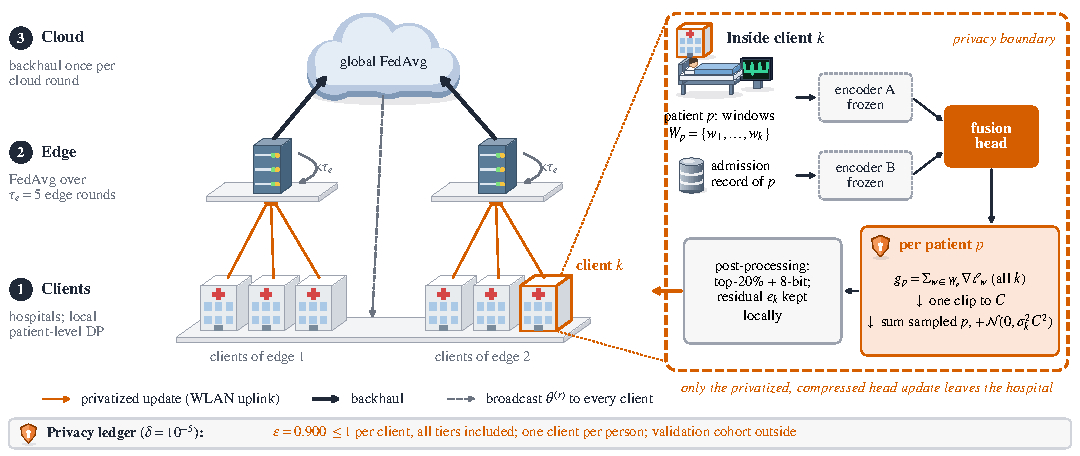
\includegraphics[width=\textwidth]{fig01_overview_core.pdf}
\caption{PP-HFM: clients train with patient-level DP, edges aggregate several
rounds locally, the cloud aggregates the edges.}
\end{figure}

\subsection{The three tiers}
\begin{description}
\item[Tier 1 -- clients (devices / hospitals).] Each holds its own patients.
It trains the model locally with patient-level DP-SGD (below) and sends a
compressed update: only the top 20\,\% of values, quantized to 8 bits, with
error feedback so nothing is permanently lost.
\item[Tier 2 -- edge servers.] Each edge averages the updates of its clients,
$\tau_e = 5$ times per cloud round. Most traffic therefore stays local and
never crosses the wide-area link.
\item[Tier 3 -- cloud.] Averages the edges once per round ($R = 10$ rounds)
and broadcasts the global model.
\end{description}

\subsection{The model}
Two encoders, one per modality (e.g.\ vital-sign time series and pre-operative
clinical variables), whose embeddings are concatenated and passed to a small
\emph{fusion head}. The model has 1.86\,M parameters; the head is 0.56\,M
(30\,\%). The encoders are pretrained once and frozen; federated training
updates only the head. All normalization layers are group/layer norm, because
batch norm mixes patients inside a batch and would break the per-patient
privacy accounting.

\subsection{Patient-level DP-SGD (the core mechanism)}
\begin{enumerate}
\item \textbf{Sample patients, not records.} Each patient is included in a step
independently with probability $q$ (Poisson sampling).
\item \textbf{Sum per patient, then clip.} All of a sampled patient's record
gradients are summed into one vector, and that vector is clipped to norm
$C = 1$. One patient can therefore move the update by at most $C$, however
many records they have.
\item \textbf{Add Gaussian noise} of scale $\sigma_k C$ and divide by the
\emph{expected} batch size $q|P_k|$ (not the realized one; see
Section~\ref{sec:fix}).
\item \textbf{Per-client noise.} Every patient belongs to exactly one client,
so each client's noise $\sigma_k$ can be calibrated to its own population
(parallel composition), instead of forcing the worst hospital's noise on
everyone. On eICU this means a median $\sigma$ of 13.4 instead of 29.3
everywhere.
\item \textbf{Accounting.} The PRV accountant computes the total
$(\varepsilon, \delta) = (0.9, 10^{-5})$ over all rounds and tiers.
\end{enumerate}

\begin{keybox}{Theorem 1 (what is proven)}
For declared public cohort sizes and fixed preprocessing, the full training
transcript of every tier is $(\varepsilon,\delta)$-DP with respect to adding or
removing one patient. It covers the \emph{training} process. It is end-to-end
only if the encoders and the standardization constants are also fitted on
public data (Section~\ref{exp:std}).
\end{keybox}

%======================================================================
\section{The data}

\begin{center}
\small
\begin{tabular}{lccc}
\toprule
& VitalDB & WEAR & eICU \\
\midrule
Domain & surgery & wearable activity & intensive care \\
Clients & 9 surgical specialties & 22 participants & 187 hospitals \\
Individuals & 6{,}257 cases & 22 & 132{,}736 \\
Records per individual ($\bar k$) & 7.8 & $\approx 1{,}750$ & 28.5 \\
Modality A & 9 vital trends + masks & inertial sensors & 6 vitals + masks \\
Modality B & 34 pre-op variables & 2048-d video features & 5 admission values \\
Task & ICU admission & 18 activities & mortality \\
Positive rate & 19.65\,\% & -- & 4.22\,\% \\
\bottomrule
\end{tabular}
\end{center}

Three choices protect the results from silent inflation: splits are by
individual (never by window); only pre-operative variables are used (the
intra-operative ones encode the outcome); missing values get an explicit
indicator channel (an arterial line is placed only in patients judged at risk,
so ``missing'' is itself informative).

On eICU a pool of 526{,}867 windows from individuals who are in no client is
reserved for pretraining the encoders, so eICU encoders never see protected
patients. On VitalDB the cohort is too small for that, so the headline uses
``oracle'' encoders pretrained on client data, which is an upper bound (the
cost of doing it properly is measured in Section~\ref{exp:f2}).

%======================================================================
\section{Experiments, one by one}

Each experiment below has the same four parts: the question, what we did,
the result, and what it means. ``Points'' means percentage points of AUROC
(0.01 AUROC = 1 point). Intervals are 95\,\% confidence intervals across seeds.

%----------------------------------------------------------------------
\begin{experiment}{System objectives on three corpora}{exp:obj}
\Q Does the full system meet the four objectives?
\D Ran the complete system on VitalDB, WEAR and eICU; network measured in NS-3
at packet level on every round, energy in CloudSim Plus, latency with ONNX
Runtime on CPU (1{,}000 runs after 100 warm-up).
\R
\begin{center}\small
\begin{tabular}{lrrrl}
\toprule
& VitalDB & WEAR & eICU & Target \\
\midrule
O1 Uplink reduction & 90.8\,\% & 96.1\,\% & 92.3\,\% & $\ge 50\,\%$ \\
O1b Round-latency cut & 16.9\,\% & 21.7\,\% & 33.4\,\% & $>0$ \\
O2a Budget $\varepsilon$ & 0.900 & 0.766 (record) & 0.900 & $\le 1$ \\
O2b Utility loss [pts] & $-0.90$ & 1.97 (inconcl.) & 3.09 (\textbf{not met}) & $\le 2$ \\
O3a P95 latency & 2.30\,ms & 0.75\,ms & 0.24\,ms & $<100$\,ms \\
O3b Update delivery & 100.00\,\% & 99.94\,\% & 97.83\,\% (\textbf{not met}) & $>99\,\%$ \\
O4 Energy saving & 72.3\,\% & 76.8\,\% & 79.6\,\% & $\ge 20\,\%$ \\
\bottomrule
\end{tabular}
\end{center}
\M Communication, latency and energy targets are met everywhere by a wide
margin. The two misses are both on eICU and both have a known cause: utility
(small hospitals, next experiments) and delivery (187 clients sharing two edges,
Section~\ref{exp:edges}).
\end{experiment}

\begin{figure}[!htb]
\centering
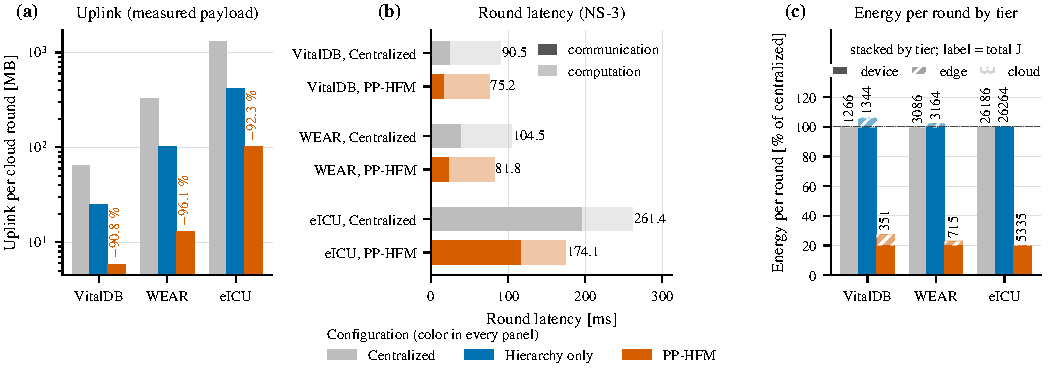
\includegraphics[width=\textwidth]{fig09_system_cost.pdf}
\caption{System cost relative to centralized training: uplink, round latency, energy by tier.}
\end{figure}

%----------------------------------------------------------------------
\begin{experiment}{Inference latency}{exp:lat}
\Q Can the model answer within 100\,ms at the edge?
\D Exported to ONNX, timed on a CPU; also tried 8-bit quantization.
\R P95 latency 2.30 / 0.75 / 0.24\,ms. On VitalDB 94\,\% of it is the forward
pass. 8-bit quantization made it \emph{slower} (P95 17.3\,ms) and broke the
WEAR GRU, so it was rejected.
\M More than a fortyfold margin. Latency is not a constraint for this model.
\end{experiment}

%----------------------------------------------------------------------
\begin{experiment}{Update delivery vs.\ number of edges (eICU)}{exp:edges}
\Q Why does eICU miss the 99\,\% delivery target?
\D Kept everything fixed and varied the number of edge servers.
\R With 2 edges, 187 clients contend for the wireless medium: 97.83\,\%
(centralized: 95.11\,\%). Delivery rises monotonically, meets 99\,\% on average
from 6 edges and in every round from 8 (about 23 clients per edge), reaching
99.94\,\% at 16.
\M It is a provisioning question, not a design flaw: the hierarchy needs
enough edges for the client count.
\end{experiment}

%----------------------------------------------------------------------
\begin{experiment}{Utility cost of privacy (O2b)}{exp:o2b}
\Q How much accuracy does $\varepsilon = 0.9$ patient-level privacy cost?
\D Identical system with and without DP, 5 paired seeds, per-client noise, PRV
accountant. AUROC is primary, because at the default 0.5 threshold the private
model predicts the majority class on every seed (accuracy = base rate), so
accuracy measures the threshold, not the model.
\R
\begin{itemize}
\item \textbf{VitalDB:} AUROC 0.8395 private vs 0.8304 non-private, change
$-0.90$ points $[-1.82, +0.02]$. No measurable cost. (Not read as ``privacy
helps'': the interval covers zero.)
\item \textbf{eICU:} 0.8245 $\rightarrow$ 0.7936, a cost of 3.09 points
$[1.37, 4.81]$. Objective not met. AUPRC cost 1.72, balanced-accuracy cost
0.50 (met). End to end (pool-fitted constants): 3.91 $[2.40, 5.42]$; all three
measures miss.
\item \textbf{WEAR} (record-level): accuracy loss 1.97\,pp $[1.76, 2.17]$; the
2-point threshold lies inside the interval, so it is inconclusive. Seeds were
fixed in advance at 15 and not extended.
\end{itemize}
\M On eICU the cost comes from the smallest hospitals: with a dozen patients
they must sample every patient at every step and carry the largest noise
multipliers (up to 29.3).
\end{experiment}

%----------------------------------------------------------------------
\begin{experiment}{Cost of the privacy unit: patient vs.\ record}{exp:unit}
\Q At the same budget, what does it cost to protect patients instead of records?
\D VitalDB, $\varepsilon = 1$, 5 paired seeds, record-level DP vs patient-level DP.
\R AUROC 0.8520 $\rightarrow$ 0.8373, a cost of 0.0147 $[0.0042, 0.0253]$;
AUPRC cost 0.0783 $[0.0532, 0.1035]$. For comparison, converting a record-level
guarantee to patients by group privacy would turn $\varepsilon = 1$ into
$\varepsilon \approx 8$; direct patient-level calibration instead needs only
1.77$\times$ more noise.
\M Protecting the right unit has a real but moderate cost. Two causes: fewer
units per step (4{,}372 patients vs 34{,}044 records), and clipping hurts
patients with many records most. The $k$-law experiments isolate the second.
\end{experiment}

\begin{figure}[!htb]
\centering
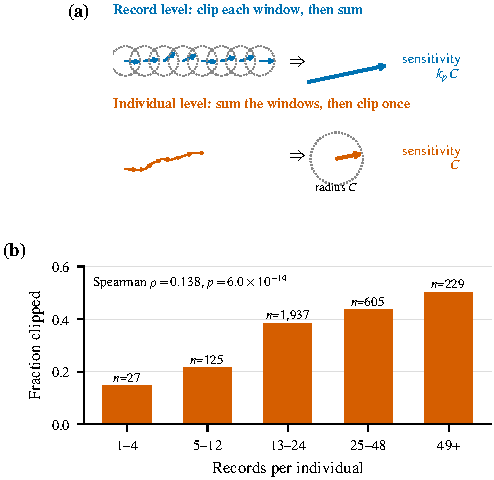
\includegraphics[width=0.55\textwidth]{fig02_privacy_unit.pdf}
\caption{Record-level vs patient-level privacy unit.}
\end{figure}

%----------------------------------------------------------------------
\begin{experiment}{What makes strict privacy survivable: initialization}{exp:init}
\Q Our recipe privatizes only the head over pretrained frozen encoders. Is
the benefit from ``head-only'' DP or from pretraining?
\D Three arms, so the two effects can be separated, at six budgets from
$\varepsilon = \infty$ to 0.5: \textbf{B4} full model, random initialization
(the usual prior art); \textbf{B7} full model, pretrained initialization;
\textbf{B6} head only, pretrained (ours).
\R (VitalDB, patient-level, 3 seeds, after the fix.)
\begin{itemize}
\item B4 $\rightarrow$ B7 (pretraining): $+0.013$ at $\varepsilon = \infty$ rising
to $+0.199$ at $\varepsilon = 0.5$; it grows at every one of the 5 steps.
\item B7 $\rightarrow$ B6 (head-only): $-0.003$ to $-0.006$, every interval
covers zero.
\item From $\varepsilon = \infty$ to 0.5 the random model loses 0.19 AUROC,
the pretrained one 0.004.
\end{itemize}
\M \textbf{Pretraining does the work; head-only DP adds nothing to accuracy.}
The effect grows exactly as privacy tightens and nearly vanishes without
privacy, a built-in dose--response. The value of head-only training is
\emph{communication}: only the head is transmitted, which is where the 90\,\%
uplink saving comes from. (Note: freezing does not reduce the noise; noise
depends on budget, steps and sampling, never on parameter count.)
\end{experiment}

\begin{figure}[!htb]
\centering
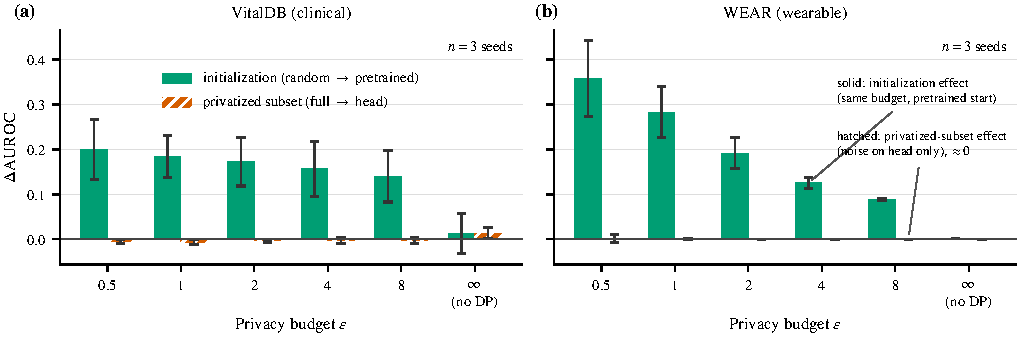
\includegraphics[width=0.85\textwidth]{fig05_init_vs_subset.pdf}
\caption{Initialization (B4$\to$B7) vs privatized subset (B7$\to$B6) across budgets.}
\end{figure}

%----------------------------------------------------------------------
\begin{experiment}{Does the hierarchy help? (component ablation)}{exp:abl}
\Q What does each component (hierarchy, DP, sparsification, quantization)
contribute?
\D Removed one component at a time; the hierarchy test was pre-registered and
run at 6 seeds.
\R Removing the hierarchy (one flat tier) changes AUROC by $-0.0047$
$[-0.0088, -0.0006]$, $p = 0.032$ on VitalDB, and $-0.0052$ $[-0.0074,
-0.0030]$, $p = 0.0018$ on WEAR, at matched $\varepsilon$. Sparsification,
quantization and loss-aware weighting are well-powered nulls on both corpora.
\M The hierarchy does not cost accuracy; removing it costs a small but
resolved 0.005. Not claimed as ``the hierarchy improves accuracy'', because the
flat arm also changes the number of local rounds. Compression is free.
\end{experiment}

%----------------------------------------------------------------------
\begin{experiment}{Does multimodal fusion help?}{exp:fusion}
\Q Does combining the two modalities beat the best single modality?
\D Fused model vs each single modality, 5 seeds; on eICU also a pre-registered
``balance'' test that degrades modality B with noise until the two modalities
are equally strong.
\R
\begin{itemize}
\item \textbf{VitalDB:} fused 0.8653 vs 0.8283, a gain of 0.0370 AUROC (5.9 seed
SD) and 0.0671 AUPRC. Resolved.
\item \textbf{WEAR:} one modality already reaches 0.9976, so there is no
headroom to test.
\item \textbf{eICU, natural:} no gain ($+0.0037$, within noise).
\item \textbf{eICU, balanced} (amendment F-A1): fused 0.7282 vs 0.6992, gain
$+0.0291$, positive on 5/5 seeds, paired $p = 0.019$ (control $+0.0020$).
\end{itemize}
\M Fusion pays when the second modality is competitive; when one modality
dominates (eICU's APACHE score), it adds nothing. An early 2-seed figure
($+0.0411$) shrank at 5 seeds; only the 5-seed figure is quoted.
\end{experiment}

%----------------------------------------------------------------------
\begin{experiment}{The $k$-law on VitalDB (records per patient)}{exp:klaw}
\Q Does the cost of patient-level privacy grow with records per patient, $k$?
\D Built training sets in which every patient has exactly $k \in \{1,2,4,8\}$
records, and trained a record-level arm and a patient-level arm with the
same units per step. 3 seeds, AUPRC primary.
\R
\begin{center}\small
\begin{tabular}{cccc}
\toprule
$k$ & Gap (record $-$ patient) & 95\,\% half-width & $p$ \\
\midrule
1 & $-0.0071$ & 0.0599 & 0.661 \\
2 & $+0.0486$ & 0.0129 & 0.004 \\
4 & $+0.0796$ & 0.0163 & 0.002 \\
8 & $+0.0872$ & 0.0248 & 0.004 \\
\bottomrule
\end{tabular}
\end{center}
The curve $A(1-1/k)$ with one parameter fits with $A = 0.1015$ (RMSE 0.0119);
a two-parameter curve does no better (0.0117). Fitted on $k \le 4$ only, it
predicts 0.0904 at $k = 8$; observed 0.0872. The patient arm is flat (0.508--0.513);
the record arm rises (0.502 $\rightarrow$ 0.596).
\M At $k = 1$ a patient is a record, so the two arms must agree; they do. That
is a built-in positive control. The growing gap is the record arm
exploiting extra records that the patient arm cannot, not the patient arm
getting worse.
\end{experiment}

\begin{figure}[!htb]
\centering
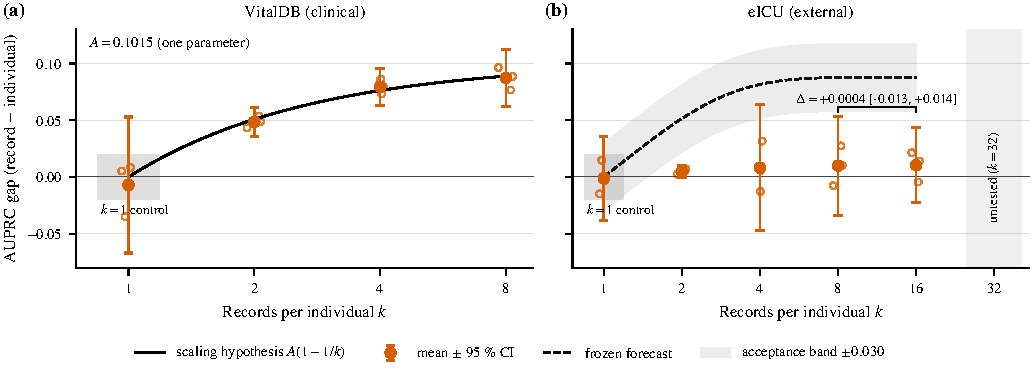
\includegraphics[width=\textwidth]{fig03_klaw.pdf}
\caption{The $k$-law: (a) VitalDB with the fitted curve; (b) eICU against the frozen forecast.}
\end{figure}

%----------------------------------------------------------------------
\begin{experiment}{External test of the $k$-law on eICU (pre-registered)}{exp:kext}
\Q Does the law transfer to a different hospital corpus?
\D Before the eICU corpus was built, we froze a forecast from VitalDB,
$\text{gap}(k) = 0.0878\,(1 - e^{-0.883(k-1)})$, with an acceptance band of
$\pm 0.030$, and extended $k$ to 16 to test saturation. ($k = 32$ was dropped
by a dated amendment before any result past $k = 8$: only 20\,\% of eICU
patients reach 32 records.)
\R (after the fix, 3 seeds)
\begin{center}\small
\begin{tabular}{cccc}
\toprule
$k$ & Gap & Forecast & $p$ \\
\midrule
1 & $-0.0011 \pm 0.0369$ & 0.0000 & 0.909 \\
2 & $+0.0048 \pm 0.0057$ & 0.0515 & 0.068 \\
4 & $+0.0081 \pm 0.0554$ & 0.0816 & 0.593 \\
8 & $+0.0099 \pm 0.0437$ & 0.0876 & 0.431 \\
16 & $+0.0103 \pm 0.0332$ & 0.0878 & 0.314 \\
\bottomrule
\end{tabular}
\end{center}
From $k = 8$ to 16 the gap changes by $+0.0004$ $[-0.0134, +0.0141]$.
\M \textbf{Shape transferred, size did not.} The control holds, the gap rises
and then flattens, as forecast. But at $k = 8$ it is about one ninth of the
forecast, and no gap is significant at three seeds (about 25 seeds would be
needed). One hypothesis: eICU's attainable precision is about half of VitalDB's
(AUPRC 0.22 vs 0.50 at 4.2\,\% prevalence). Distinguishing that from a
corpus-specific ceiling needs a third corpus. Seeds are \emph{not} being added
to chase significance.
\end{experiment}

%----------------------------------------------------------------------
\begin{experiment}{Is the eICU shortfall just the budget? (matched grid)}{exp:matched}
\Q The forecast was fitted at $\varepsilon = 1$, batch 32; eICU ran at 0.8,
batch 64. Is that why eICU is smaller?
\D Re-ran the VitalDB $k$-grid at the eICU operating point.
\R The VitalDB gaps do not shrink ($+0.0914$ vs $+0.0872$ at $k = 8$). But this
grid fails its own $k = 1$ control ($+0.0398$, all seeds the same sign),
probably from the smallest pool combined with the largest batch. Correcting
every grid for its own $k = 1$ offset attributes about half (51\,\%) of the
$k = 8$ difference to the operating point.
\M Under either reading the budget does not explain the factor of nine, and
the corpus effect never changes sign.
\end{experiment}

%----------------------------------------------------------------------
\begin{experiment}{Is the cost an artefact of the clipping rule?}{exp:clip}
\Q Clipping a patient's \emph{summed} gradient hurts patients with many
records. Would normalizing by record count before clipping recover the cost?
(It changes nothing about the privacy guarantee.)
\D Three rules: fixed bound, divide by $k$, divide by $\sqrt{k}$. Pre-registered
criterion: count normalization must recover at least $+0.010$ AUPRC.
\R
\begin{itemize}
\item \textbf{eICU, before the fix:} change $-0.0001$; the one-sided upper
bound $+0.0058$ excludes $+0.010$. Fails.
\item \textbf{VitalDB at $k = 8$, after the fix (D1):} clipped fraction falls
from 0.50 to 0.34, AUPRC changes by $+0.0038$ $[-0.0072, +0.0148]$; the upper
bound $+0.0113$ does \emph{not} exclude $+0.010$: \textbf{inconclusive} by its
own rule, though even the bound is one eighth of the 0.0914 cost.
\item \textbf{eICU, after the fix (D2):} final-round clipped fraction falls
from 0.14 to 0.08, AUPRC changes by $-0.0012$ $[-0.0093, +0.0069]$; the upper
bound $+0.0043$ excludes $+0.010$. \textbf{Fails} (as before the fix). The
square-root rule changes AUPRC by $-0.0031$.
\end{itemize}
\M Normalization changes how often clipping binds but not accuracy. On eICU
the clipping rule does not explain the cost; on VitalDB it could explain at
most one eighth of it. The cost belongs mainly to the patient unit itself.
\end{experiment}

%----------------------------------------------------------------------
\begin{experiment}{Privacy audit: membership inference (LiRA)}{exp:mia}
\Q Can an attacker tell whether a \emph{patient} was in training, and does
patient-level DP leak less than record-level DP?
\D LiRA attack with 16 shadow models per arm, 5 target seeds, 4 attacks. A
positive control (a no-DP model known to memorize) had to pass first.
\R (after the fix, stage E2) Positive control AUC 0.623, 0.060 above its
difficulty floor: the attack works. Record-level DP 0.548, patient-level DP
0.524 (only 0.008 above its floor). Record minus patient, paired over 5 seeds:
loss $+0.012$ $[-0.006, +0.030]$, offline LiRA $+0.029$ $[-0.038, +0.095]$,
online LiRA $-0.003$ $[-0.015, +0.009]$; online LiRA with global variance
$-0.029$ $[-0.048, -0.010]$ ($p = 0.014$), i.e.\ the record arm leaks
\emph{less}, which does not survive correction for four attacks.
\M The large predicted difference (0.7 vs 0.5) is refuted. A small difference
is not excluded at this sample size. The attack works (control passes), so
the null is meaningful.
\end{experiment}

%----------------------------------------------------------------------
\begin{experiment}{Private conformal prediction (negative result)}{exp:conf}
\Q Can each client release a private calibration threshold so that the
system outputs prediction sets with 90\,\% coverage?
\D Exponential-mechanism quantile per client ($\varepsilon_{\text{conf}} = 0.1$),
aggregated by edges and cloud; coverage measured on the test split.
\R Thresholds land mid-range (0.42--0.61). The private model's probabilities sit
near zero, so every set is just the majority class: coverage equals the base
rate (80.1\,\% on VitalDB, fails; 95.7\,\% on eICU), and \emph{no positive
patient is covered}.
\M With about 100 calibration patients per client at $\varepsilon = 0.1$, the
mechanism cannot separate thresholds. Conformal prediction was therefore
removed from the system and the contributions, and the full budget
$\varepsilon = 0.9$ goes to training. It stays in the paper as an honest
negative result.
\end{experiment}

%----------------------------------------------------------------------
\begin{experiment}{Standardization constants: a hidden release}{exp:std}
\Q Input normalization means and SDs are fitted on training patients. Do they
leak?
\D Measured, exactly, how much one patient can move them (leave-one-out over
92{,}909 eICU individuals), and compared them with constants fitted on the
public pool.
\R Removing one patient moves any mean by at most 0.0017 SD; for 99\,\% of
patients any SD by at most 0.02\,\%; but one outlier moves one channel's SD by
5.2\,\%. Pool-fitted constants differ by at most 0.026 SD and 4.4\,\%.
\M Small, but it is a release outside the guarantee. Fix: re-standardize
eICU with pool-fitted constants (verified exact: the stored data reproduce the
original constants to $4\times10^{-8}$), re-pretrain the encoders and re-run.
That run is the only configuration that is private end to end.
\R AUROC 0.8209 $\rightarrow$ 0.7819, a cost of 3.91 points $[2.40, 5.42]$
($p = 0.002$, 5 seeds); AUPRC 2.66 $[1.82, 3.49]$; balanced accuracy 2.69
$[1.57, 3.82]$.
\M Public constants make the guarantee end to end and cost about 0.8 AUROC
points more than training-fitted ones (3.09); now all three measures miss the
2-point target.
\status{done 29 Oct.}
\end{experiment}

%----------------------------------------------------------------------
\begin{experiment}{Cost of disjoint encoders on VitalDB (F2)}{exp:f2}
\Q How much does it cost to pretrain VitalDB's encoders on a disjoint pool
instead of on client data?
\D Stage F2: the headline patient-level run on VitalDB repeated with encoders
pretrained only on the disjoint pool, five seeds, private and non-private arms.
\R Against the oracle encoders the private model loses 0.0157 $\pm$ 0.0046
AUROC (0.8395 $\to$ 0.8237, $p < 0.001$) and 0.0122 $\pm$ 0.0262 AUPRC (not
resolved). With disjoint encoders the cost of privacy itself is $+0.0014$
$[-0.0033, +0.0062]$ AUROC and $+0.0221$ $[-0.0003, +0.0446]$ AUPRC.
(Before the fix, record-level: 0.0322 AUROC, 0.0763 AUPRC.)
\M Honest encoders cost about 1.6 AUROC points on VitalDB, half the earlier
estimate. Standardization constants are still fitted on client data here, so
this run is not end to end; only the eICU re-run with public constants is.
\end{experiment}

%======================================================================
\section{Mistakes found and fixed}\label{sec:fix}

A large part of this project was finding errors that produced
plausible-but-wrong numbers without any crash. Each one was fixed, tested,
and the affected results re-run. The important ones:

\begin{center}
\small
\begin{tabular}{p{0.32\textwidth} p{0.6\textwidth}}
\toprule
Error & Effect and fix \\
\midrule
Noise calibrated from one client & Every DP arm exceeded its budget.
Now calibrated against all clients. \\
Conformal calibration fired 5$\times$ & Total $\varepsilon$ was 3.49, not 0.96.
Fixed to fire once; later removed entirely. \\
NS-3 had never run & Every early ``network result'' was an analytical
fallback. NS-3 built; packet-level every round. \\
Stale partition metadata & Noise calibrated on wrong counts. Rebuilt. \\
eICU training collapse & Model decayed to constant output in long epochs,
which would have poisoned every eICU $k$-number. Fixed validation cadence. \\
Divided by the realized batch $|S|$ (22 Oct) & Not the analysed mechanism;
at small hospitals it reveals the patient count. Now divides by the expected
batch. All patient-level results re-run in stages A--G. \\
Headline runs were record-level & The system runs used record-level DP
while claiming patient-level. Re-run at patient level. \\
Aggregation weights leaked sizes & Now static declared sizes. \\
\bottomrule
\end{tabular}
\end{center}

\begin{warnbox}{Why this matters}
Every one of these would have survived review unnoticed and would have broken
the central claim. The paper's numbers are all from the corrected code; the old
results are archived, not overwritten.
\end{warnbox}

%======================================================================
\section{Honest scorecard: what is and is not claimed}

\begin{center}
\small
\begin{tabular}{p{0.5\textwidth} l}
\toprule
Claim & Status \\
\midrule
Patient-level guarantee for hierarchical multimodal FL, all tiers accounted & proven (Theorem 1) \\
Communication, latency, energy objectives & met on all three corpora \\
No measurable utility cost on VitalDB at $\varepsilon = 0.9$ & supported \\
Utility cost $\le 2$ points on eICU & \textbf{not met} (3.09; 3.91 end to end) \\
Pretrained initialization makes strict privacy survivable & strongly supported \\
Head-only DP improves accuracy & \textbf{refuted} (it helps communication) \\
$k$-law shape on VitalDB & supported, with positive control \\
$k$-law transfers to eICU & shape yes, magnitude no, unresolved \\
Cost is not a clipping artefact & eICU yes; VitalDB inconclusive ($\le 1/8$ of cost) \\
Patient DP leaks much less than record DP (MIA) & large effect refuted \\
Private conformal prediction & \textbf{failed}, removed \\
Fusion helps & VitalDB yes; eICU only when balanced \\
Hierarchy costs accuracy & no (removing it costs 0.005) \\
\bottomrule
\end{tabular}
\end{center}

None of the building blocks is new (user-level DP, private fine-tuning,
hierarchical FL). The contribution is their composition inside a hierarchy
with a proof, and careful \emph{measurement} of what it costs.

%======================================================================
\section{Still to do}

\begin{center}
\begin{tabular}{lll}
\toprule
Item & What it gives & Expected \\
\midrule
HED-FL, FL2DP baselines & empirical comparison & needs the two PDFs \\
Final consistency pass & paper ready to submit & after numbers freeze \\
\bottomrule
\end{tabular}
\end{center}

Your decisions: the journal (IEEE IoT Journal or TII), authors, bios,
acknowledgment, and a final reference check.

%======================================================================
\section{Glossary}
\begin{description}
\item[Federated learning (FL)] Training where data stays at each site and only
model updates are shared.
\item[Hierarchical FL] FL with an intermediate edge tier that aggregates nearby
clients before the cloud.
\item[Differential privacy ($\varepsilon$, $\delta$)] A guarantee that the output
barely changes whether or not one unit's data is included. Smaller
$\varepsilon$ is stronger; $\varepsilon \le 1$ is considered strong.
\item[Privacy unit] What the guarantee protects: one record, or one patient.
\item[DP-SGD] Training with per-unit gradient clipping and Gaussian noise.
\item[Clipping norm $C$] The maximum size of one unit's contribution.
\item[Noise multiplier $\sigma$] Noise scale relative to $C$.
\item[Accountant (PRV, RDP)] Computes the total $\varepsilon$ over all steps.
\item[AUROC / AUPRC] Ranking quality of the model; AUPRC is more sensitive
when positives are rare (eICU: 4.2\,\%).
\item[Seed] One independent repetition of a training run; paired seeds compare
two arms on identical splits.
\item[Pre-registration] Writing down the prediction and the pass/fail rule
before running the experiment, so the result cannot be reinterpreted later.
\item[LiRA] Likelihood-ratio membership-inference attack using shadow models.
\item[Oracle vs disjoint encoders] Pretrained on client data (upper bound, not
private) vs on a separate public pool (private end to end).
\end{description}

\end{document}
